\section{Prácticos realizados}
\subsection{BCD $\rightarrow$ Exceso-3}
\textbf{Consigna:}
Diseñar y armar un conversor de código BCD a XS3 (exceso 3). Realizar: \begin{enumerate} \item Tabla de verdad \item Obtener las funciones lógicas de calidas con circuitos combinacionales. \item Minimizar el circuito y verificar su funcionamiento en el MiniLab. \item Armar el circuito y verificar su funcionamiento en el simular ''falstad.com'' \end{enumerate}

\subsection{Comparador binario}

El siguiente circuito es un comparador binario de dos números $A$ y $B$ de dos bits cada uno. Las salidas ($S0$, $S1$ y $S2$) representan la salida del comparador y cuando $S0 = 1$ cuando $A>B$ y $S2 = 1$ para $A = B$, en caso de no darse la condición, la salida permanece en cero.

\begin{center}
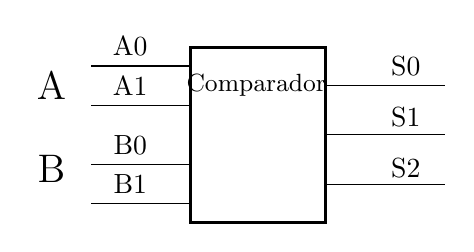
\begin{tikzpicture}
	\node[shape=rectangle, draw, line width=1pt, inner sep=0, minimum width=1.715cm, minimum height=2.215cm] at (5.125, 3.125){};
	\draw (4.25, 4) -- (3, 4);
	\draw (4.25, 3.5) -- (3, 3.5);
	\draw (4.25, 2.25) -- (3, 2.25);
	\draw (4.25, 2.75) -- (3, 2.75);
	\draw (6, 2.5) -- (7.5, 2.5);
	\draw (6, 3.75) -- (7.5, 3.75);
	\draw (6, 3.125) -- (7.5, 3.125);
    \node at (3.5, 4.25) {A0};
    \node at (3.5, 3.75) {A1};
    \node at (3.5, 3) {B0};
    \node at (3.5, 2.5) {B1};
    \node at (7, 4) {S0}; 
    \node at (7, 3.35) {S1};
    \node at (7, 2.7) {S2};
    \node at (5.1 , 3.75) {\small Comparador};
    \node at (2.5, 3.75) {\Large A};
    \node at (2.5, 2.7) {\Large B};
\end{tikzpicture} \end{center}

Se pide:
\begin{enumerate} \item Tabla de verdad. \item Obtener las funciones lógicas de salidas con circuitos combinacionales. \item Circuito mínimo usando mapa de Karnaugh. \item Circuito mínimo usando teoremas y postulados de álgebra de Boole. \item Armado de circuito y verificado en MiniLab. \item Armado de circuito y verificado con simulador ''falstad.com'' \end{enumerate}

\section{Cálculos y respuestas}
\subsection{Exceso 3}
\begin{itemize} \item Tabla de verdad: \end{itemize}

\begin{center}
\begin{tabular}{|llll|llll|}
\hline
\rowcolor[HTML]{FFCE93} 
\multicolumn{1}{|c}{\cellcolor[HTML]{FFCE93}\textbf{A}} & \multicolumn{1}{c}{\cellcolor[HTML]{FFCE93}\textbf{B}} & \multicolumn{1}{c}{\cellcolor[HTML]{FFCE93}\textbf{C}} & \multicolumn{1}{c|}{\cellcolor[HTML]{FFCE93}\textbf{D}} & \multicolumn{1}{c}{\cellcolor[HTML]{FFCE93}\textbf{W}} & \multicolumn{1}{c}{\cellcolor[HTML]{FFCE93}\textbf{X}} & \multicolumn{1}{c}{\cellcolor[HTML]{FFCE93}\textbf{Y}} & \multicolumn{1}{c|}{\cellcolor[HTML]{FFCE93}\textbf{Z}} \\ \hline
0                                                       & 0                                                      & 0                                                      & 0                                                       & 0                                                      & 0                                                      & 1                                                      & 1                                                       \\
0                                                       & 0                                                      & 0                                                      & 1                                                       & 0                                                      & 1                                                      & 0                                                      & 0                                                       \\
0                                                       & 0                                                      & 1                                                      & 0                                                       & 0                                                      & 1                                                      & 0                                                      & 1                                                       \\
0                                                       & 0                                                      & 1                                                      & 1                                                       & 0                                                      & 1                                                      & 1                                                      & 0                                                       \\
0                                                       & 1                                                      & 0                                                      & 0                                                       & 0                                                      & 1                                                      & 1                                                      & 1                                                       \\
0                                                       & 1                                                      & 0                                                      & 1                                                       & 1                                                      & 0                                                      & 0                                                      & 0                                                       \\
0                                                       & 1                                                      & 1                                                      & 0                                                       & 1                                                      & 0                                                      & 0                                                      & 1                                                       \\
0                                                       & 1                                                      & 1                                                      & 1                                                       & 1                                                      & 0                                                      & 1                                                      & 0                                                       \\
1                                                       & 0                                                      & 0                                                      & 0                                                       & 1                                                      & 0                                                      & 1                                                      & 1                                                       \\
1                                                       & 0                                                      & 0                                                      & 1                                                       & 1                                                      & 1                                                      & 0                                                      & 0                                                       \\
1                                                       & 0                                                      & 1                                                      & 0                                                       & X                                                      & X                                                      & X                                                      & X                                                       \\
1                                                       & 0                                                      & 1                                                      & 1                                                       & X                                                      & X                                                      & X                                                      & X                                                       \\
1                                                       & 1                                                      & 0                                                      & 0                                                       & X                                                      & X                                                      & X                                                      & X                                                       \\
1                                                       & 1                                                      & 0                                                      & 1                                                       & X                                                      & X                                                      & X                                                      & X                                                       \\
1                                                       & 1                                                      & 1                                                      & 0                                                       & X                                                      & X                                                      & X                                                      & X                                                       \\
1                                                       & 1                                                      & 1                                                      & 1                                                       & X                                                      & X                                                      & X                                                      & X                                                       \\ \hline
\end{tabular}
\end{center}

\begin{itemize} \item Obtención de funciones lógicas \end{itemize}

\ecuacion{Z = \sum (0; 2; 4; 6; 8)}
\ecuacion{Y = \sum (0; 3; 4; 7; 8)}
\ecuacion{X = \sum (1; 2; 3; 4; 9)}
\ecuacion{W = \sum (5; 6; 7; 8; 9)}

\begin{center}
\begin{Karnaugh}
    \contingut{0,1,1,1,1,0,0,0,X,X,X,X,0,1,X,X}
   % \implicant{1}{3}{red}
   % \implicant{2}{3}{green}
   % \implicant{5}{15}{purple}
   \implicantdaltbaix[3pt]{3}{10}{blue}
   \implicantdaltbaix[3pt]{1}{11}{red}
   \implicant{4}{12}{green}
    % \implicantcantons[2pt]{orange}
   % \implicantcostats{4}{14}{green}
\end{Karnaugh} \end{center}
\begin{center}
\begin{Karnaugh}
    \contingut{1,0,1,1,1,0,1,1,1,0,X,X,X,X,X,X}
   \implicantcostats{0}{10}{green}
   \implicant{3}{11}{red}
\end{Karnaugh} \end{center}
\begin{center}
\begin{Karnaugh}
    \contingut{0,0,0,0,0,1,1,1,1,1,X,X,X,X,X,X}
    \implicant{12}{10}{red}
    \implicant{5}{15}{blue}
    \implicant{7}{14}{green}
\end{Karnaugh} \end{center}

\midTitle{red}{Funciones}
$Z = \overline{D}$ \\
$Y = C.D+\overline{C}.\overline{D}$ \\
$X = D.\overline{B} + C.\overline{B} + \overline{C}.\overline{D}.B$ \\
$W = A + B.D + B.C$ \\
\inicioCodigo{}

\finalCodigo{}
